\section{Background and Motivation}

\subsection{Long-Tail Effect in RL Rollouts}
RL algorithms such as PPO~\cite{schulman2017proximal} and GRPO~\cite{guo2025deepseek} typically follow a synchronized iterative cycle: (1) \textit{rollout}, (2) \textit{reward calculation}, and (3) \textit{actor update}. Among these, the rollout phase is most time-consuming, often accounting for over 70\% of total training time and thus becoming the primary bottleneck in RL training~\cite{he2025history_rhyme, hu2025taming}. 

In the rollout phase, the policy model usually samples multiple responses for a batch of prompts across distributed data-parallel (DP) ranks. 
A key challenge arises from the inherent variance in generation length, due to both the stochastic nature of sampling and prompt diversity. This variability induces severe long-tail effects, especially in long-context RL training, leading to GPU idleness (called \textit{bubbles}). More specifically, these bubbles can be divided into two categories: (1) \textbf{Inter-GPU Bubbles.} DP ranks that finish all assigned prompts must wait for the slowest rank to complete, leaving some GPUs completely idle, as illustrated in \autoref{fig:bubble} left part. (2) \textbf{Intra-GPU Bubbles.} Within a DP rank, most generations have relatively short responses and terminate early, so the remaining computation proceeds with a much smaller effective batch size. In this case, GPUs are not fully idle, but their utilization is low, as shown in the right part of \autoref{fig:bubble}. These bubbles can account for more than $60\%$ of the total rollout time, making the rollout phase GPU-inefficient and difficult to scale.

To mitigate these bubbles, prior work has explored relaxing synchronization constraints. Techniques such as asynchronous RL~\cite{fu2025areal} decouple rollout workers from the actor update, enabling continuous response generation with minimal synchronization overhead for weight updates. However, these methods inevitably introduce response staleness, which can destabilize RL training, as increasingly noted in recent studies~\cite{xi2026jet, qi2025defeating, liuspeed}. Given the crucial importance of maintaining synchrony, our work instead aims to accelerate the rollout phase by leveraging these inevitable bubbles without compromising the synchronous property.

\noindent $\blacktriangleright$ \textbf{\underline{Insight}:} Rather than eliminating bubbles, \model proactively exploits them to pre-generate rollouts, forming \textbf{cross-batch pipelining for RL training}. To avoid the distributional mismatch between generation and training, \model uses these responses for suffix-tree-based speculative decoding to accelerate LLM inference.

% Directly using these pre-generated rollouts for the next policy update causes a distribution mismatch between generation and training. Instead, \model uses these responses for suffix-tree-based speculative decoding to accelerate LLM inference.

\begin{figure}[t!]
    \centering
    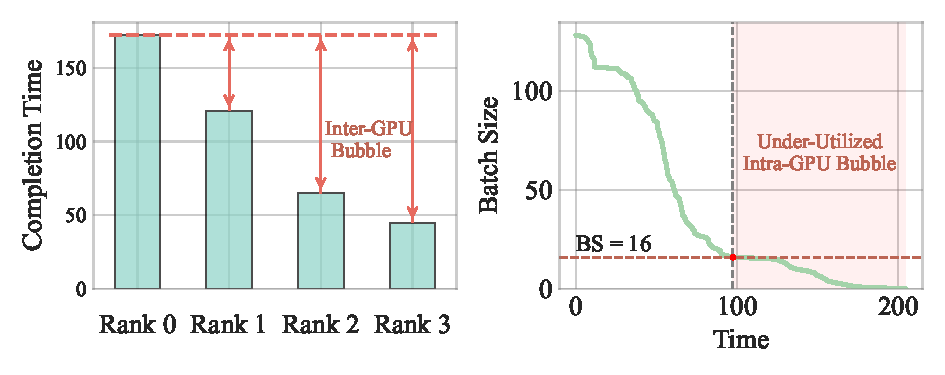
\includegraphics[width=1.0\linewidth]{figures/gpu_bubble.pdf}
    \caption{Inter‑GPU and intra‑GPU bubbles in RL rollouts}
    \label{fig:bubble}
\end{figure}
\subsection{Model-Free Speculative Decoding} 
\label{sec:spec_decoding}

Speculative decoding~\cite{leviathan2023fast} accelerates LLM inference via a draft-then-verify paradigm: it first generates draft tokens using a lightweight method, then verifies them in parallel with the target model. 
Crucially, rejection sampling ensures that the final output distribution is mathematically identical to standard auto-regressive sampling~\cite{leviathan2023fast}. 

While speculative decoding greatly reduces the number of forward calls of the target model, \ie decode steps, the per-step latency may increase due to two factors: (1) \textbf{Draft overhead}, the additional time needed to generate draft tokens; and (2) \textbf{Verification overhead}, the increased target-model forward latency caused by a larger and varying-length batch. Assuming the decoding-step reduction ratio and per-step latency increase ratio are $\alpha$ and $\mu$, respectively, the end-to-end generation time reduction ratio is
% 
\begin{equation}
\text{Speedup} = 1 - (1-\alpha)(1+\mu).
\end{equation}
% 
Model-based speculative methods incur substantial draft overhead, causing their acceleration to deteriorate at the large batch sizes typical of RL rollouts~\cite{li2025eagle3}. In contrast, model-free approaches typically generate draft tokens via prefix pattern matching within existing sequences, achieving much lower draft overhead.
Consequently, recent work has explored model-free approaches to accelerate RL rollouts~\cite{he2025history_rhyme, liu2025specRL}. These methods typically exploit inter-epoch similarity by reusing rollouts from the previous epoch as drafts for the current epoch. While promising, they are mainly validated with training on small-scale datasets and exhibit two major limitations. 
First, they provide \textbf{no acceleration during the initial epoch}, which is a critical bottleneck in large-scale training where a single epoch may span hundreds or thousands of steps and last days or even weeks. 
Second, as the dataset size and the steps per epoch increase, the \textbf{policy model can change drastically between epochs}. 
This divergence reduces the relevance of historical rollouts, degrading draft quality and diminishing speculative speedup.

\noindent $\blacktriangleright$ \textbf{\underline{Insight}:} 
Our key intuition is to \textbf{leverage per-step rollout bubbles to generate drafts for subsequent steps}, while keeping draft and verification overhead low, thereby achieving consistent speedup throughout the training process.
